\documentclass{beamer}
%
% Choose how your presentation looks.
%
\usepackage[T1]{fontenc}
\usepackage[utf8]{inputenc}
\usepackage{lmodern}  
\usepackage{tikz}%boxy s vysvetlivkami 
\usetikzlibrary{calc}
\usepackage{amsmath}
\usepackage{bm}
%
% For more themes, color themes and font themes, see:
% http://deic.uab.es/~iblanes/beamer_gallery/index_by_theme.html
%
\mode<presentation>
{
  \usetheme{Darmstadt}      % or try Darmstadt, Madrid, Warsaw, ...
  \usecolortheme{default} % or try albatross, beaver, crane, ...
  \usefonttheme{serif}  % or try default, serif, structurebold, ...
  \setbeamertemplate{navigation symbols}{}
  \setbeamertemplate{caption}[numbered]
} 
%
%
\title[Week1]{Week 3:  Lag Operators \\ Cointegration (continued), Forecasting}
\author{Advanced Econometrics 4EK608}
\institute{Vysoká škola ekonomická v Praze}
\date{}

\begin{document}
 
\begin{frame}
  \titlepage
\end{frame}

% Uncomment these lines for an automatically generated outline.
\begin{frame}{Outline}
  \tableofcontents
\end{frame}

%
\section{Czech terminology}

\begin{frame}{Czech terminology}
Operátory zpoždění
\\ Superkonzistence
\\ Grangerův reprezentační teorém
\\ Engle-Grangerova dvoustupňová procedura
\\ Kointegrační vektor 
\end{frame}

%---------------------------------------------
\section{Stationarity of ar($p$) processes}

\begin{frame}{Lag operators}
Lag operators:
\begin{align*}
Lx_t &= x_{t-1} \\
L(Lx_t)=L^2x_t &= x_{t-2} ~~~~~~~~~~~~~~~~~\\
&\cdots \\
L^p x_t &= x_{t-p} 
\end{align*}

Using lag operators,
$$ AR(p):  x_t = \alpha + \phi_1 x_{t-1} + \phi_2 x_{t-2} +\dots + \phi_p
  x_{t-p}+u_t$$
can be rewritten as: 
$$(1-\phi_1 L - \phi_2 L^2 - \dots - \phi_p L^p)x_t = \alpha + u_t $$

\end{frame}

%---------------------------------------------

\begin{frame}{Stationarity}
\vspace{-0.5cm}
\begin{equation} \label{eq1}
(1-\phi_1 L - \phi_2 L^2 - \dots - \phi_p L^p)x_t = \alpha + u_t
\end{equation}

Stochastic process \eqref{eq1} will only be stationary if the roots of corresponding equation \eqref{eq2}  are all greater than unity in absolute value 
\vspace{-0.5cm}
\begin{equation} \label{eq2}
1-\phi_1 L - \phi_2 L^2 - \dots - \phi_p L^p = 0
\end{equation}
\vspace{-0.5cm}
\begin{block}{Illustration 1 - AR(1) process:}
\vspace{-0.5cm}
\begin{align}
\vspace{-0.5cm}
x_t & =  \alpha + \phi x_{t-1} + u_t \label{eq3}  \\ \nonumber
(1-\phi L) x_t & =  \alpha + u_t\\ \nonumber
~ \\ \nonumber
1- \phi L & = 0 \\ \nonumber
L & = 1/\phi \\ \nonumber
\textnormal{For \eqref{eq3} to be stationary} &, \textnormal{$|L|>1 \leftrightarrow -1 < \phi < 1$}
\end{align}
\end{block}

\end{frame}

%---------------------------------------------

\begin{frame}{Stationarity}
\begin{block}{Illustration 2:}
\begin{equation}
x_t   = 2 + 3.9 x_{t-1} + 0.6 x_{t-2} - 0.8 x_{t-3} + u_t \label{eq4}
\end{equation}
To evaluate stationarity of $x_t$, we use
\begin{equation*}
1-3.9 L - 0.6 L^2 + 0.8 L^3  = 0 , 
\end{equation*}
which can be factorized:
$$ (1-0.4L)(1+0.5L)(1-4L) =0 $$
\vspace{-0.5cm}
\begin{align} \notag
1^{st} root: & L = 2.5 \\ \notag
2^{nd} root: & L =-2 \\ \notag
3^{rd} root: & L = 0.25 \Rightarrow \textnormal{\eqref{eq4}  is non-stationary}
\end{align}
\end{block}
\end{frame}

%---------------------------------------------

\section{Cointegration}

\begin{frame}{Cointegration between two variables}
\textbf{Superconsistency:} $y_t =  \beta_0 + \beta_1 x_t + u_t$\\
\begin{enumerate}
\item Provided $x_t$ and $y_t$ are cointegrated, the OLS estimators $\hat{\beta}_0$ and $\hat{\beta}_1$ will be consistent. 
\item $\hat{\beta}_j$ converge in probability to their true values $\beta_j$ more quickly in the cointegrated non-stationary case than in the stationary case (asymptotic efficiecy).
\end{enumerate}
\begin{block}{Consequences:}
For simple static regression between two cointegrated variables: $y_t, x_t \sim C(1,1)$, super-consistency applies (with deterministic regressors such as intercept and trend added upon relevance). Dynamic misspecifications do not necessarily have serious consequences. This is a large sample property - in small samples, OLS estimators are biased.\\ (Specific statistical inference applies to cointegrating vectors.)
\end{block}
\end{frame}

%---------------------------------------------

\begin{frame}{Cointegration between two variables}
\textbf{Granger representation theorem:}\footnote{Engle and Granger (1987)}\\
If two TS $x_t$ and $y_t$ are cointegrated, the short-term disequilibrium relationship between them can be expressed in the ECM form
\vspace{-0.2cm}
\begin{equation} \label{eq6}
 \Delta y_t = lagged(\Delta y, \Delta x) - \delta u_{t-1} + \varepsilon_t 
\end{equation}
where $u_{t-1} = y_{t-1} - \beta_0 - \beta_1 x_{t-1}$ is the disequilibrium error and $\delta$ is a short-run adjustment parameter. \\
\footnotesize{Note: as $u$ is on the scale of $y$, $\delta$ can be interpreted in percentages. Example: $\delta = +0.8 \rightarrow 80 \%$ of the disequilibrium error gets corrected between $t-1$ and $t$ (on average).}
\vspace{0.1cm}

\textbf{Two implications:}
\begin{enumerate}
\item The general-to-specific model search can focus on ECMs
\item Engle-Granger two-stage procedure
\end{enumerate}
\end{frame}

%---------------------------------------------

\begin{frame}{Cointegration between two variables}
\textbf{Engle-Granger two-stage procedure:}

\medskip
We short-cut the search of an ECM from a general model
\begin{itemize}
\item[ $1^{st}$ ]  stage: Estimation of the cointegrating (static) regression and saving residuals $$\hat{u}_t = y_t - \hat{\beta}_0 - \hat{\beta}_1 x_t$$
\item [$2^{nd}$]  stage: Use residuals $\hat{u}_{t-1}$ in \eqref{eq6} instead of $u_{t-1}$ and estimate by OLS
\end{itemize}
Estimator are consistent and asymptotically efficient, but biased in small samples. 

\medskip
\small{Assumptions: $y_t$ and $x_t$ are non-stationary and cointegrated.}
\end{frame}

%---------------------------------------------

%slide 9
\begin{frame}{Cointegration among more than two variables}
\textbf{Possibility of more cointegrating vectors}\\
long-run: $y_t= \beta_0 + \beta_1 x_t + \beta_2 w_t + \beta_3 z_t + u_t$,\\ all observed variables are $I(1)$\\
\medskip
If this long-run relationship exists, then the disequilibrium error \\
\begin{equation}  \label{eq7}
u_t= [y_t - \beta_0 - \beta_1 x_t - \beta_2 w_t - \beta_3 z_t ]
\quad \sim I(0) 
\end{equation} 

\vspace{0.3cm}
In the multivariate case, there may be more then one stationary linear combination linking cointegrated variables. 

\vspace{0.3cm}
If a linear combination of variables such as \eqref{eq7} is stationary, then the coefficients in this relationship form a cointegrating vector, e.g. $(1,-\beta_{1},-\beta_{2},-\beta_{3})$. 

\vspace{0.3cm} 
Cointegration: the existence of at least one cointegrating vector.

\end{frame}

%---------------------------------------------

%slide 10
\begin{frame}{Cointegration among more than two variables}
\textbf{Testing and estimation}\\
Cointegration can be tested using the EG and/or PO tests

\hspace{0.3cm}

\textbf{Only one cointegrating vector exists}\\
Estimation can proceed by the Engle-Granger two-stage method for ECMs. \\ 
\vspace{0.3cm}
\textbf{More than one cointegrating vectors}\\
Engle-Granger two-stage method is not applicable. Johansen (1988) suggests a maximum likelihood approach. 
\end{frame}

%---------------------------------------------

\section{Predictions - basics}

\begin{frame}{Predictions - basics}
\begin{itemize}
\item LRM and its estimate:
\begin{align}\nonumber
y & = \beta_0 + \beta_1 x_1 +\beta_2 x_2 + \dots + \beta_k x_k + u\\ \nonumber
\hat{y} & = \hat{\beta}_0 + \hat{\beta}_1 x_1 +\hat{\beta}_2 x_2 + \dots + \hat{\beta}_k x_k \\ \nonumber
\end{align}
\item Prediction of expected value: 
\begin{align}\nonumber
\hat{y}_p & = E(y|x_1 = c_1, x_2 = c_2,\dots,x_k = c_k)\\ \nonumber
\hat{y}_p & = \hat{\beta}_0 + \hat{\beta}_1 c_1 +\hat{\beta}_2 c_2 + \dots + \hat{\beta}_k c_k  \nonumber
\end{align}
\item Rough (underestimated) confidence interval for the expected value prediction: (95\%): $\hat{y}_p \pm 2 \times \textit{s.e.}(\hat{y}_p)$. \\ (Rule of thumb) 
\end{itemize}
\end{frame}

%---------------------------------------------

\begin{frame}{Predictions - basics}
$\textit{s.e.}(\hat{y}_p)$ can be obtained by reparametrization:

\vspace{0.5cm}
\begin{itemize}
\item Reparametrized LRM:
$$y^*=\beta^*_0 + \beta^*_1 (x_1 -c_1) + \beta^*_2(x_2 - c_2) + \dots + u$$
\item The following holds:
\begin{align} \nonumber
 \hat{y}_p &= \hat{\beta_0^*} \\ \nonumber
 \textit{s.e.}(\hat{y}_p ) &= 
   \textit{s.e.}(\hat{\beta_0^*}), \hspace{0.2cm} i.e. \\ \nonumber
 Var(\hat{y}_p) &= Var(\hat{\beta}_0^*)
\end{align} 
\end{itemize}
\end{frame}

%---------------------------------------------

\begin{frame}{Predictions - basics}
\begin{itemize}
\item Predicted and actual values of $y_p$:
\begin{align}\nonumber
\hat{y}_p &  = \hat{\beta}_0 + \hat{\beta}_1 c_1 + \hat{\beta}_2 c_2 + \dots + \hat{\beta}_k c_k\\ \nonumber
y_p & = \beta_0 + \beta_1 c_1 + \beta_2 c_2 + \dots+\beta_k c_k + u_p \nonumber
\end{align} 
\item Prediction error
$$\hat{e}_p = y_p - \hat{y}_p = (\beta_0 + \beta_1 c_1 + \beta_2 c_2 + \dots+\beta_k c_k) + u_p - \hat{y}_p$$
\item Prediction error variance
$$Var(\hat{e}_p) = Var(u_p) + Var(\hat{y}_p)$$
because $Var(\beta_0 + \beta_1 c_1 + \beta_2 c_2 + \dots+\beta_k c_k)=0$
\end{itemize}
\end{frame}

%---------------------------------------------

\begin{frame}{Predictions - basics}
\begin{itemize}
\item If homoskedasticity holds, $\sigma^2 = Var(u_p)$: \\

\begin{itemize}
\item $Var(\hat{e}_p) = \sigma^2 + Var(\hat{y}_p)$
\vspace{0.2cm}
\item We estimate $\sigma^2$ from the original LRM as $(\textit{SSR}/(n-k-1))$
\vspace{0.2cm}
\item We get $Var(\hat{y}_p)$ from the reparametrized LRM
\end{itemize}
\vspace{0.5cm}
\item Standard prediction error:
\begin{itemize}
\vspace{0.2cm}
 \item $\textit{s.e.}(\hat{e}_p) = \sqrt[]{Var(\hat{e}_p)}$
\end{itemize}
\vspace{0.5cm}
\item Prediction interval (95\%)
\vspace{0.2cm}
\begin{itemize}
\item $\hat{y}_p \pm t_{0.025} \times \textit{s.e.}(\hat{e}_p) $
\end{itemize}
\end{itemize}
\end{frame}

%---------------------------------------------

\begin{frame}{Predictions - basics}
\begin{itemize}
\item Prediction with logarithmic dependent variable
\begin{align}\nonumber
\log(y) &= \beta_0 + \beta_1 x_1 + \dots + \beta_k x_k + u\\\nonumber
\widehat{\log(y)} &= \hat{\beta}_0 + \hat{\beta}_1 x_1 + \dots + \hat{\beta}_k x_k 
\end{align}
$\hat{y} =e^{\widehat{\log(y)}}$ systematically underestimates $\hat{y}$ , \\
\vspace{0.3cm}
we can use a correction: $\hat{y}=\widehat{\alpha}_0 e^{\widehat{\log(y)}}$ \\
\vspace{0.3cm}
where $\widehat{\alpha}_0 = n^{-1} \sum_{i=1}^n \exp(\hat{u}_i)$ \\
\vspace{0.3cm}
is a consistent (not unbiased) estimator of $\exp{(u)}$.
\end{itemize}
\end{frame}

%---------------------------------------------
\begin{frame}{Predictions - basics (Matrix form)}
Prediction based on estimated model:\\
\vspace{0.3cm}
$\hat{y}_p = \bm{x}_{p}^\prime \hat{\bm{\beta}}$\\
\vspace{0.3cm}
Difference between prediction and actual $y_p$ value:\\
\vspace{0.3cm}
$\hat{e}_p \,=\, \hat{y}_p - y_p
  \,=\, \bm{x}_{p}^\prime \hat{\bm{\beta}} - \bm{x}_{p}^\prime \bm{\beta} - u_p
  \,=\, \bm{x}_{p}^\prime (\hat{\bm{\beta}} - \bm{\beta}) - u_p$\\
\vspace{0.3cm}
If $\hat{\bm{\beta}}$ is unbiased estimator for $\bm{\beta}$, \\
$\hat{y}_p$ is an unbiased estimator for $y_p$ value:\\
\vspace{0.3cm}
$E(\hat{e}_p) \,=\, E(\hat{y}_p - y_p)
   \,=\, \bm{x}_{p}^\prime E(\hat{\bm{\beta}} - \bm{\beta}) + E(-u_p) =0$\\
\vspace{0.3cm}
and the variance of $\hat{e}_p$ can be expressed as:\\
\vspace{0.3cm}
$E(\hat{e}_p^2) \,=\,\textit{var}(\hat{e}_p)
   \,=\, \bm{x}_{p}^\prime \textit{var}(\hat{\bm{\beta}})\bm{x}_{p} + \textit{var}(u_p) $
\end{frame}

%---------------------------------------------

\begin{frame}{Predictions - basics (Matrix form)}
Variance of $\hat{e}_p$ (continued):
\begin{equation*}
\begin{aligned}
\textit{var}(\hat{e}_p) \,&=\,
  \bm{x}_{p}^\prime \textit{var}(\hat{\bm{\beta}})\bm{x}_{p} + \textit{var}(u_p)\\
 \,&=\,
   \bm{x}_{p}^\prime \left[ \sigma^2 \left( \bm{X}^\prime \! \bm{X}  \right)^{-1} \right] \bm{x}_{p} + \textit{var}(u_p)\\
   & \textnormal{substitute $\sigma^2, \textit{var}(u_p)$ with $\hat{\sigma}^2$ (homoskedasticity)}\\
  \,&=\,
   \underbrace{\bm{x}_{p}^\prime \left[ \hat{\sigma}^2 \left( \bm{X}^\prime \! \bm{X}  \right)^{-1} \right] \bm{x}_{p}}_{\hat{\sigma}_p^2}
   + \hat{\sigma}^2
\end{aligned}
\end{equation*}
With growing sample size (asymptotically), \\
$\textit{var}(u_p) = \hat{\sigma}_p^2 + \hat{\sigma}^2$ converges to $\hat{\sigma}^2$\\
$\dots$ $\textit{plim} \, \hat{\bm{\beta}} = \bm{\beta} \,\,\,\, \Rightarrow \,\,\,\, 
  \textit{plim} \, \hat{\sigma}_p^2 = 0$

\end{frame}

%---------------------------------------------
\begin{frame}{Predictions - basics (Matrix form)}
Variance of $\hat{e}_p$ (continued):
\begin{equation*}
\begin{aligned}
\textit{var}(\hat{e}_p) \,&=\,
\bm{x}_{p}^\prime \left[ \hat{\sigma}^2 \left( \bm{X}^\prime \! \bm{X}  \right)^{-1} \right] \bm{x}_{p}
   + \hat{\sigma}^2\\
   & \textnormal{after re-arranging, $s.e.(\hat{e}_p)$ may be written as}\\
   &~\\
   s.e.(\hat{e}_p) \,&=\, \hat{\sigma} \cdot \,  
   \sqrt[]{1+ \bm{x}_{p}^\prime \left( \bm{X}^\prime \! \bm{X}  \right)^{-1} \bm{x}_{p}~} \,,\\
   &\textnormal{which relates to the individual prediction error. }\\
   &\textnormal{For mean prediction errors (considering $\hat{\sigma}_p^2$ only): }\\
   s.e.(\widetilde{e}_p) \,&=\, \hat{\sigma} \cdot \,  
   \sqrt[]{~~~~ \bm{x}_{p}^\prime \left( \bm{X}^\prime \! \bm{X}  \right)^{-1} \bm{x}_{p}~} \,.\\
\end{aligned}
\end{equation*}

\end{frame}

%---------------------------------------------
\begin{frame}{Predictions - basics (Matrix form)}
Prediction intervals: individual vs. mean value predictions:\\
\vspace{0.3cm}
\textbf{Individual prediction:} $y_p \in \hat{y}_p \pm t^*_{\alpha/2} \times s.e.(\hat{e}_p)$\\
\vspace{0.3cm}
\textbf{Mean value:} \hspace{1.7cm} $y_p \in \hat{y}_p \pm t^*_{\alpha/2} \times s.e.(\widetilde{e}_p)$

\begin{figure}
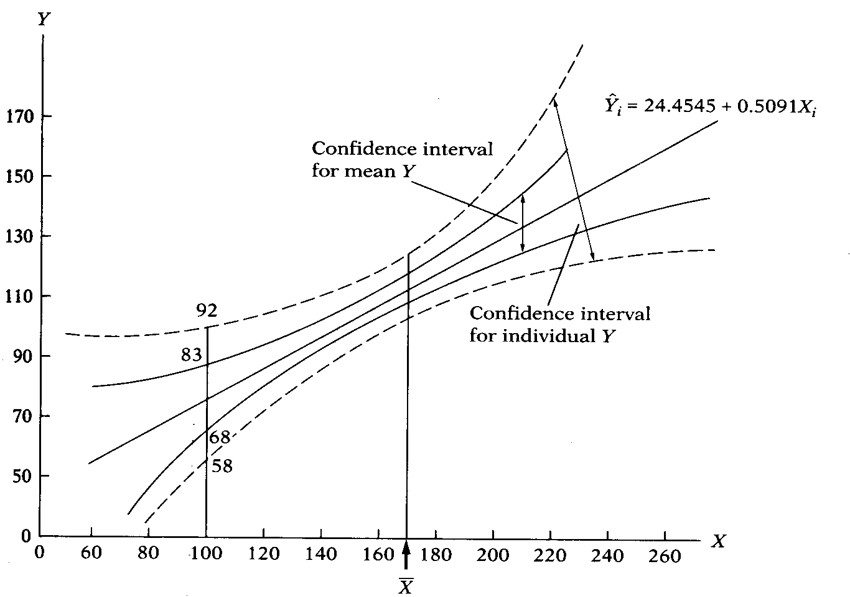
\includegraphics[width=0.6\textwidth]{img/P3_PredError.jpg}
\end{figure}

\end{frame}

%---------------------------------------------
\begin{frame}{Predictions - basics}
\begin{itemize}
\item Why is it difficult to predict individual values? 
\begin{itemize}
\item they include random errors
\item we work with estimated parameters
\item parameters can change in time
\item (look at the formula for prediction error.)
\end{itemize}
\vspace{0.3cm}
\item Prediction of expected values
\begin{itemize}
\item parameters are estimated
\item parameters can change in time
\end{itemize}
\vspace{0.3cm}
\item Impacts of random errors on predictions of individual values are usually much bigger than the impacts of (variance in) estimated parameters.
\end{itemize}
\end{frame}
%---------------------------------------------
\section{Variance vs. Bias trade-off}

\begin{frame}{Mean Squared Error of prediction}

We can generalize the previous discussion on predictions by considering both biased and unbiased predictors and by allowing for different functional forms and complexity levels in predictive models. Predictions may be compared using:

\medskip
\begin{itemize}
   \item $\textit{MSE} = \textnormal{E}
   \left[y_i - \hat{f}(\bm{x}_i) \right]^2$\\
   \smallskip
   where $\hat{f}(\bm{x}_i)$ is the prediction that $\hat{f}$ generates for the $i$-th regressor set. $\hat{f}$ represents a general class of predictors (linear, non-linear, non-parametric, etc.) and it may produce either biased or unbiased predictions
\end{itemize}
\end{frame}
%---------------------------------------------
\begin{frame}{Variance vs. Bias trade-off}
Population equation example: $~y = \textnormal{sin}(x)+u$
\vspace{-1 cm}
\begin{figure}
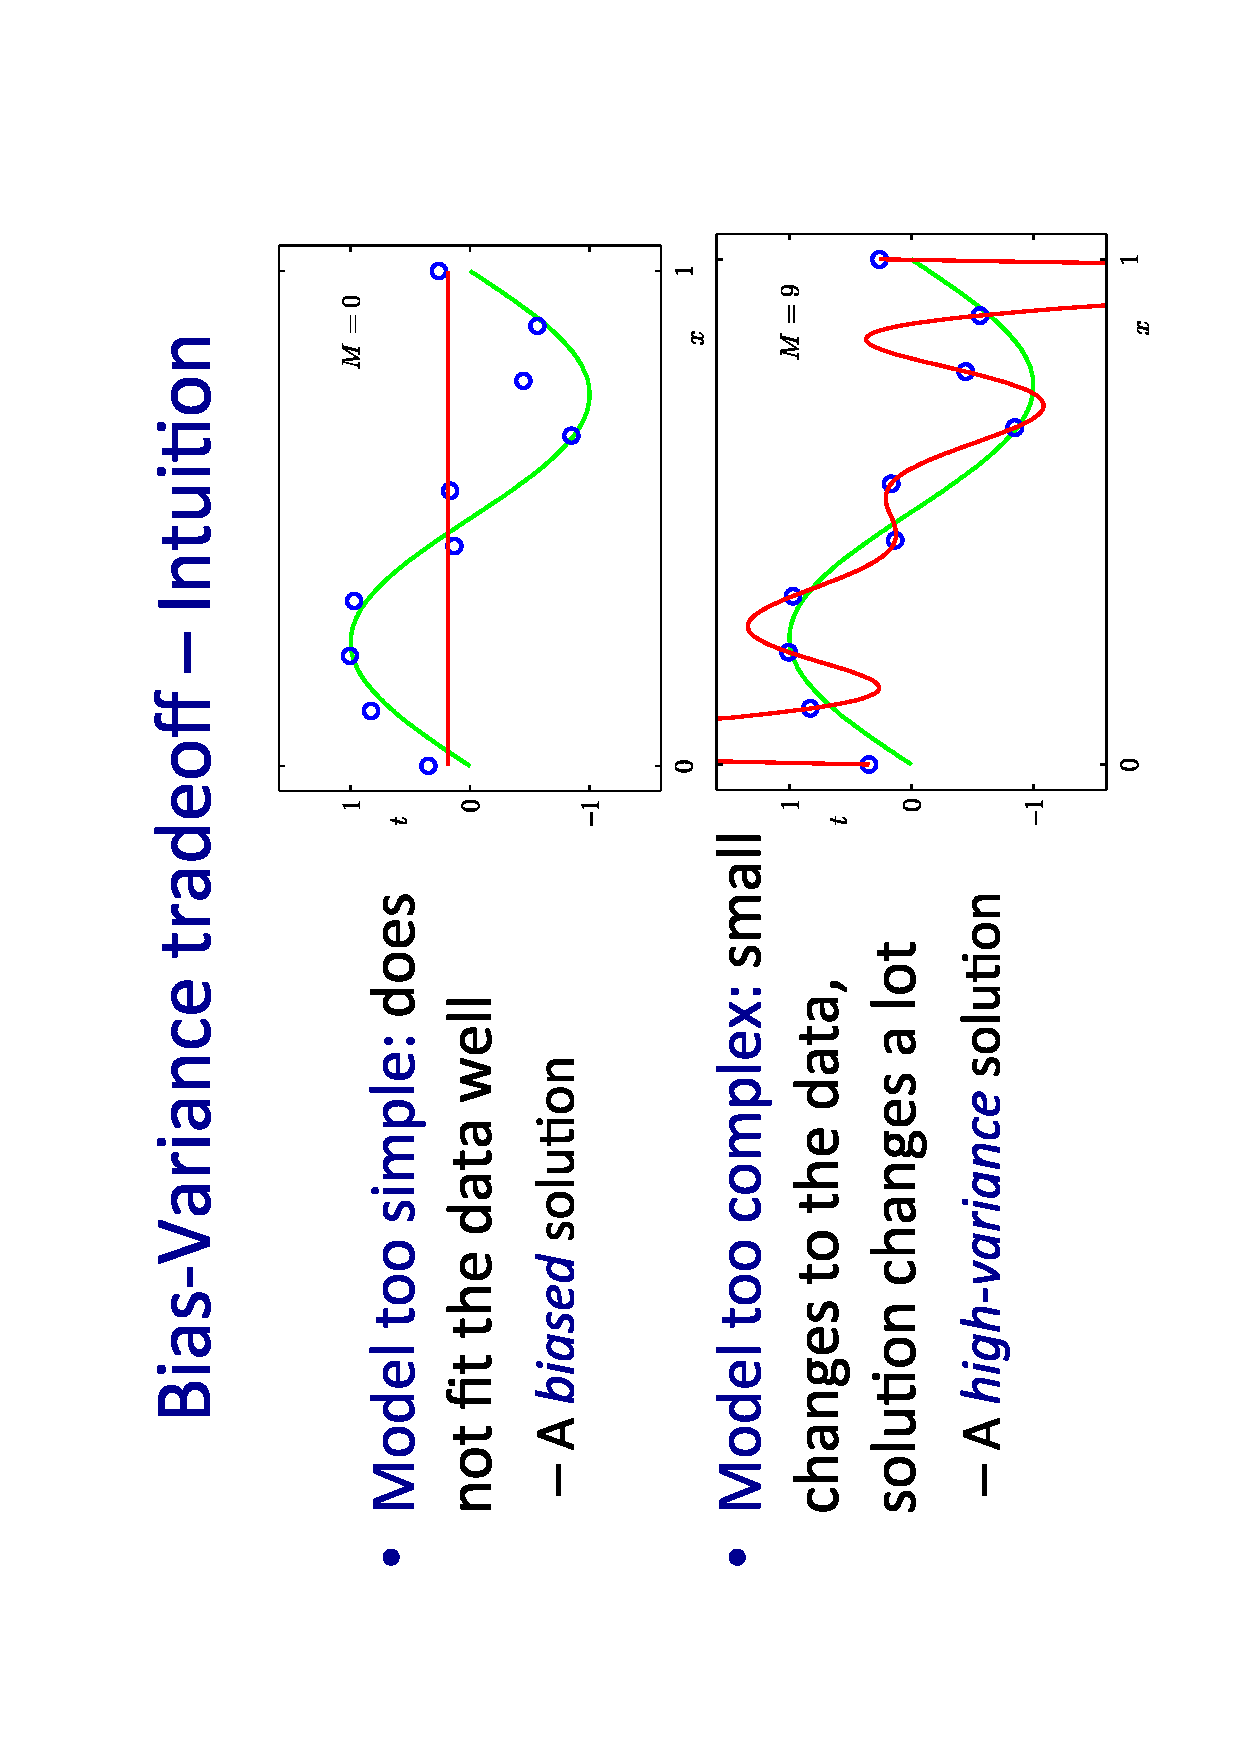
\includegraphics[angle=270,scale=0.35]{img/VarBias.pdf}
\end{figure}
\end{frame}
%---------------------------------------------
\begin{frame}{Train sample \& Test sample}

Suppose we fit a model $\hat{f}(\bm{x})$ to some training data $\textnormal{Tr}=\left\lbrace y_i, \bm{x}_i \right\rbrace _1 ^n$ and we wish to see how well it performs.

\begin{itemize}
\item We could compute $\textit{MSE}$ over $\textnormal{Tr}$:
$$ \textit{MSE}_{\textnormal{Tr}} = \frac{1}{n}
   \sum_{i \in \textnormal{Tr}}
   \left[y_i - \hat{f}(\bm{x}_i) \right]^2 $$
\end{itemize}

When searching for the ``best'' model by minimizing $ \textit{MSE}$, the above statistic would lead to over-fit models.
\vspace{0.3 cm}
\begin{itemize}
\item Instead, we should (if possible) compute the $ \textit{MSE}$ using fresh test
data $\textnormal{Te}=\left\lbrace y_i, \bm{x}_i \right\rbrace _1 ^m$:
$$ \textit{MSE}_{\textnormal{Te}} = \frac{1}{m}
    \sum_{i \in \textnormal{Te}}
   \left[y_i - \hat{f}(\bm{x}_i) \right]^2 $$
\end{itemize}
\end{frame}
%------------------------------------------------
\begin{frame}{Variance vs. Bias trade-off}

Suppose we have a model $\hat{f}(\bm{x})$, fitted to some training data $\textnormal{Tr}$ and let $\left\lbrace y_0, \bm{x}_0 \right\rbrace$ be a test observation drawn from the population. If the true model is $y_i = f(\bm{x}_i) + \varepsilon_i$, \\[with $f(\bm{x}_i)= \textnormal{E}(y_i | \bm{x}_i )$],
then the \textbf{expected test MSE} can be decomposed into:\\
\medskip
$\textnormal{E}(\textit{MSE}_0)
   = Var(\hat{f}(\bm{x}_0))
   + [Bias(\hat{f}(\bm{x}_0))]^2
   + \textit{var}(\varepsilon_0),$

where\\
\smallskip
$Bias(\hat{f}(\bm{x}_0)) 
       = \textnormal{E}[\hat{f}(\bm{x}_0)]
       - f(\bm{x}_0)$,\\
$\varepsilon_0$ is the irreducible error: $\textnormal{E}(\textit{MSE}_0) \geq \varepsilon_0$,\\ 
all three RHS elements are non-negative,
\smallskip
\\The above equation refers to the average test $\textit{MSE}$ that we would obtain if we repeatedly estimated $f(\bm{x})$ using a large number of training sets and then tested each $\hat{f}(\bm{x})$ at $\bm{x}_0$.
\end{frame}
%---------------------------------------------
\begin{frame}{Variance vs. Bias trade-off}
$\textnormal{E}(\textit{MSE}_0)
   = Var(\hat{f}(\bm{x}_0))
   + [Bias(\hat{f}(\bm{x}_0))]^2
   + \textit{var}(\varepsilon_0),$\\
\begin{figure}
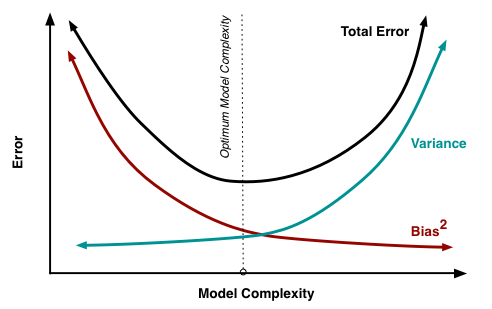
\includegraphics[angle=0,scale=0.35]{img/biasvariance.png}
\end{figure}
\end{frame}
%------------------------------------------------
\section{$k$-Fold Cross Validation}
\begin{frame}{$k$-Fold Cross Validation}
\begin{itemize}
\item Training error ($\textit{MSE}_{\textnormal{Tr}}$) can be calculated easily. 
\item However, $\textit{MSE}_{\textnormal{Tr}}$ is not a good approximation for the $\textit{MSE}_{\textnormal{Te}}$ (out-of sample predictive properties of the model).
\item Usually, $\textit{MSE}_{\textnormal{Tr}}$ dramatically underestimates $\textit{MSE}_{\textnormal{Te}}$.
\end{itemize}
\bigskip
Cross-validation is based on re-sampling (similar to bootstrap).\\
\medskip
Repeatedly fit a model of interest to samples formed from the training set \& make ``test sample'' predictions, in order to obtain additional information about predictive properties of the model.\\
\end{frame}
%---------------------------------------------
\begin{frame}
\frametitle{$k$-Fold Cross Validation}

\begin{itemize}
  \item In $k$-Fold Cross-Validation ($k$FCV), the original sample is randomly partitioned into $k$ roughly equal subsamples (divisibility). 
  \item Of the $k$ subsamples, a single subsample is retained as the test sample, and the remaining $(k-1)$ subsamples are used as training data. 
  \item The cross-validation process is then repeated $k$ times (the $k$ folds), with each of the $k$ subsamples used exactly once as the test sample. 
  \item The $k$ results from the folds can then be averaged to produce a single estimation. 
  \item $k = 5$ or $k=10$ is commonly used.
\end{itemize}  
\end{frame}
%------------------------------------------------
\begin{frame}{$k$-Fold Cross Validation}
\begin{center}
$k$FCV example for $k=5$: \\
(random sampling, no replacement)
\begin{figure}
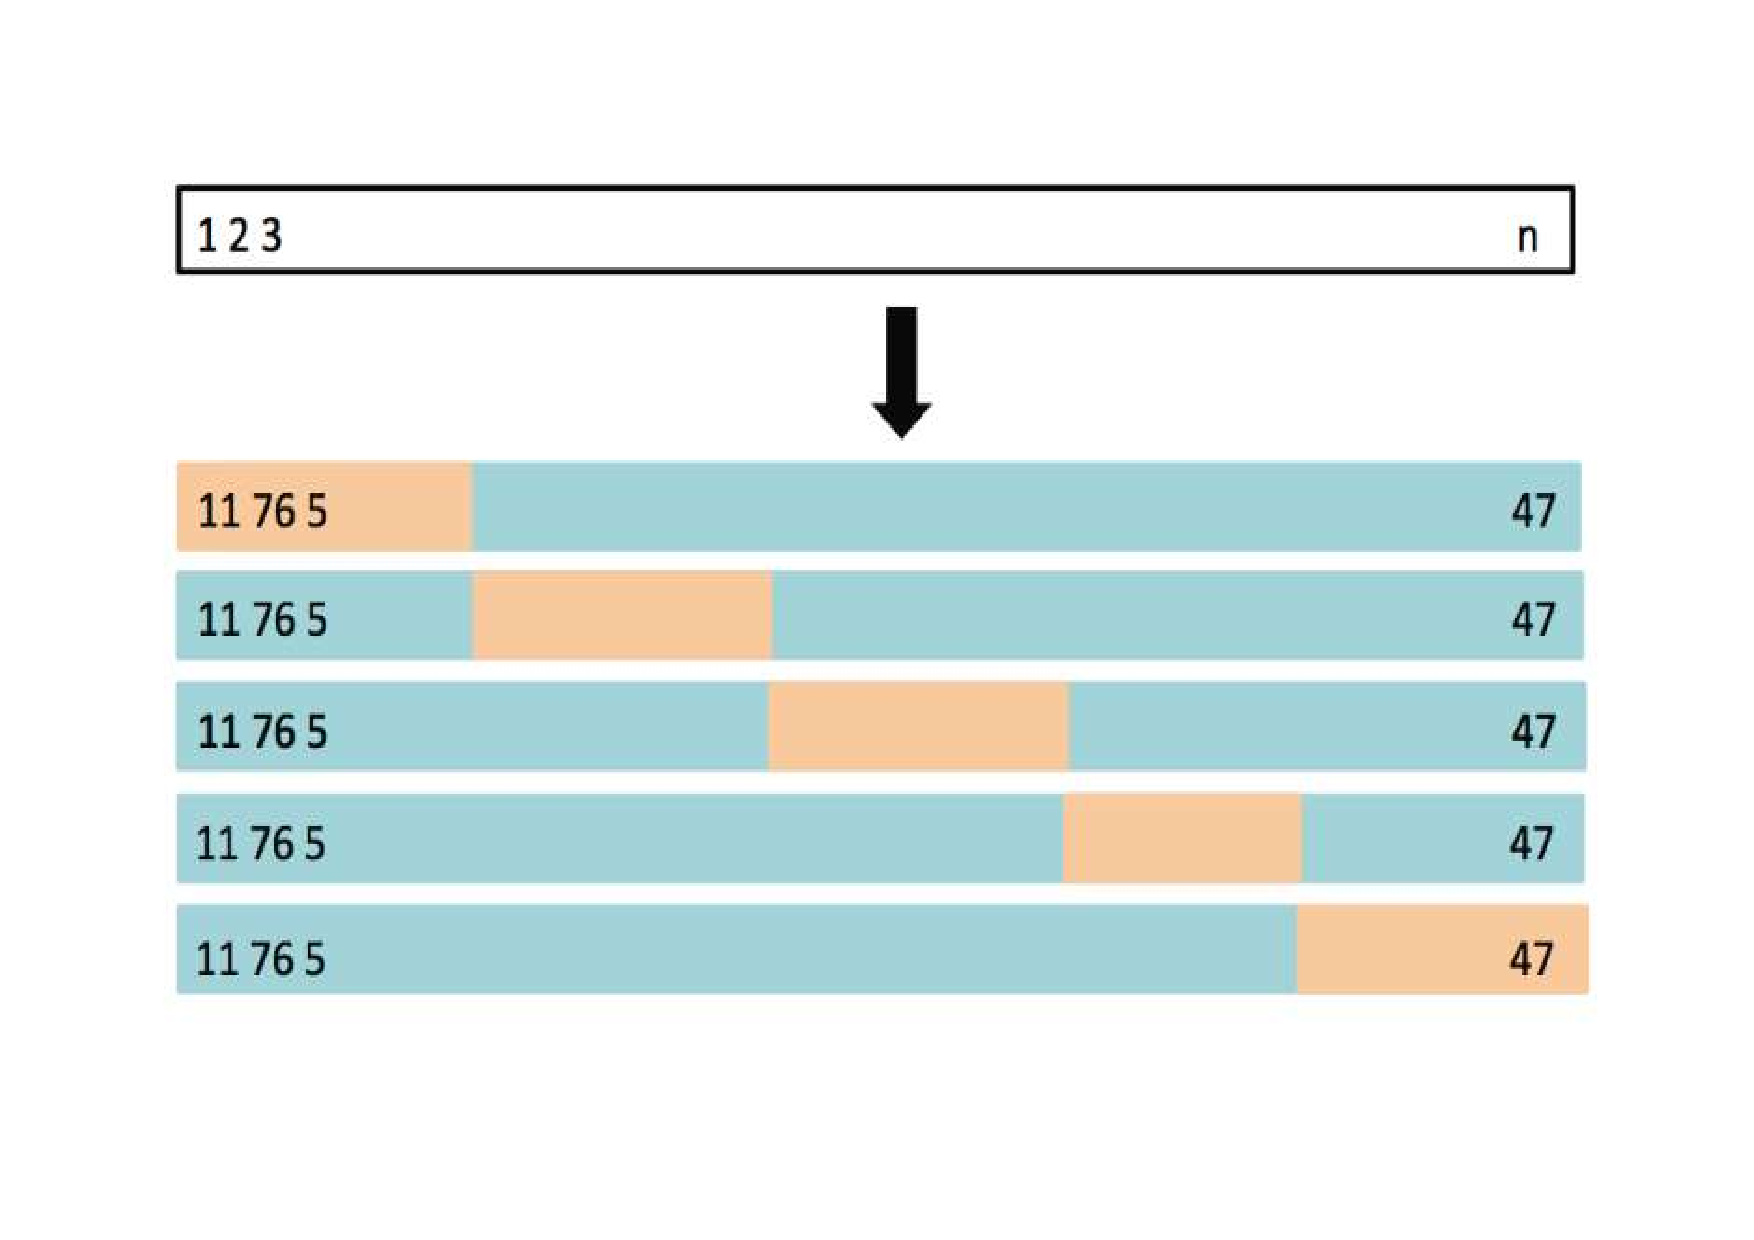
\includegraphics[width=0.7\linewidth]{img/kFCV2.pdf}
\end{figure}
\end{center}
\end{frame}
%------------------------------------------------
\begin{frame}{$k$-Fold Cross Validation}
$ \textit{CV}_{(k)}= \frac{1}{k}\displaystyle\sum_{s=1}^{k} \textit{MSE}_s ,$
\vspace{0.3cm}
\begin{itemize}
\item [where] $\textit{CV}_{(k)}$ is the $k$-fold \textit{CV} estimate,
\item [ ] $k$ is the number of folds used (e.g. 5 or 10),
\item [ ] $\textit{MSE}_s = \frac{1}{m_s} \sum_{i \in C_s}^{}(y_i - \widehat{y}_i)^2 $ 
\item [ ] $m_s$ and $C_s$ refer to test sample  observations for each \\of the $k$ train sample / test sample steps.
\end{itemize}
\vspace{0.3cm}
As we compare predictions from two or more models, 
\\we look for the lowest $\textit{CV}_{(k)}$. 
\end{frame}
%---------------------------------------------
\section{Chow tests}
\begin{frame}{Chow tests}
Focus on DGP stability \& model suitability for predictions.

\medskip
For any LRM: $\bm{y} = \bm{X\beta}+\bm{u}$
\vspace{0.3cm}
\begin{itemize}
\item Chow tests are used to determine whether the regression function differs for different time periods \\(or respondent groups in CS data). 
\item Time-stability of the estimated coefficients is a necessary condition for forecasting from an estimated model.
\item Groups can be formed by different time periods.

\item Chow tests can be defined for cross-sectional units as well. \\(wages for male/female individuals, etc.)
\end{itemize}

\end{frame}

%---------------------------------------------


\begin{frame}{Chow tests}

For any LRM: $\bm{y} = \bm{X\beta}+\bm{u}$
\vspace{0.3cm}

\begin{itemize}

\item Say, the sample (time series) for a period $t=1,2, \dots, T$ may be conveniently divided into two groups: $T_1 + T_2 = T$.  \\ 
$[$ consider two periods: fixed vs. floating F/X rates $]$ \\ 
$[$ pre-EU accession vs. post-EU accession period $]$
\vspace{0.3cm}
\item Now, the LRM's vectors and matrices may be partitioned as follows: \\
\vspace{0.3cm}
$ \begin{bmatrix} \bm{y}_1 \\ \bm{y}_2 \end{bmatrix} = 
\begin{bmatrix} \bm{X}_1 \\ \bm{X}_2 \end{bmatrix} \bm{\beta} +
\begin{bmatrix} \bm{u}_1 \\ \bm{u}_2 \end{bmatrix}$ \\
\vspace{0.2cm}
where $\bm{y}_1^\prime = (y_1, \dots , y_{T_1})$, 
$\bm{y}_2^\prime = (y_{T_1+1}, \dots , y_{T})$, etc. 
\\ i.e. $\left\lbrace\bm{y}_1, \bm{X}_1 \right\rbrace \in T_1$,  
$\left\lbrace\bm{y}_2, \bm{X}_2 \right\rbrace \in T_2$. 

\end{itemize}

\end{frame}



%---------------------------------------------


\begin{frame}{Chow tests}

For any LRM: $\bm{y} = \bm{X\beta}+\bm{u}$, Chow test can be based on an auxiliary regression (unrestricted model for the $F$ test):
\vspace{0.3cm}

\begin{itemize}

\item 
$ \begin{bmatrix} \bm{y}_1 \\ \bm{y}_2 \end{bmatrix} = 
\begin{bmatrix} \bm{X}_1 \\ \bm{X}_2 \end{bmatrix} \bm{\beta} +
\begin{bmatrix} \bm{0} \\ \bm{X}_2 \end{bmatrix} \bm{\gamma} +
\begin{bmatrix} \bm{u}_1 \\ \bm{u}_2 \end{bmatrix}$ \\
\vspace{0.3cm}
where $\bm{0}$ is a zero-matrix of the same dimensions as $\bm{X}_1$, 
\\ i.e. $(T_1 \! \times \! k)$.
\end{itemize}

Also, we can see that:

\begin{itemize}

\item 
$ T_1: \hspace{0.5cm} \hat{\bm{y}}= \bm{X} \bm{\hat{\beta}}  $ 
\item 
$ T_2: \hspace{0.5cm} \hat{\bm{y}}= \bm{X} 
  ( \bm{\hat{\beta}} + \bm{\hat{\gamma}} ) $ 

\end{itemize}

Note: Power of the test depends on proper $T_1$ vs. $T_2$ cutoff. 
\\ Chow test may be generalized for 3+ time periods (groups).

\end{frame}




%---------------------------------------------



\begin{frame}{Chow tests}

For  our unrestricted model:
\vspace{0.3cm}

\begin{itemize}

\item 
$ \begin{bmatrix} \bm{y}_1 \\ \bm{y}_2 \end{bmatrix} = 
\begin{bmatrix} \bm{X}_1 \\ \bm{X}_2 \end{bmatrix} \bm{\beta} +
\begin{bmatrix} \bm{0} \\ \bm{X}_2 \end{bmatrix} \bm{\gamma} +
\begin{bmatrix} \bm{u}_1 \\ \bm{u}_2 \end{bmatrix}$ \\
\vspace{0.3cm}
\end{itemize}

We can formulate the null of no structural change in model dynamics between the two time periods (groups) as follows:

\begin{itemize}
\item 
$ H_0: \hspace{0.5cm} \bm{\gamma}= \bm{0}$, i.e.: 
$\gamma_0 = \gamma_1 = \gamma_2= \cdots = \gamma_k=0 $
\item 
$ H_1: \hspace{0.5cm} \neg H_0$ 
\end{itemize}

This can be tested using an $F$-test (or its HC version): 
\vspace{0.3cm}
\begin{itemize}
\item 
$ F = \frac{\textit{SSR}_r- \textit{SSR}_{\textit{ur}}}{\textit{SSR}_{\textit{ur}}} \times \frac{n-2k}{k} \underset{H_0}{\sim } 
F[k, (n-2k)] $ 
\end{itemize}



\end{frame}



%---------------------------------------------


\begin{frame}{Chow test - Example}
A simple Chow test example for CS data: 
\\(to assess whether parameters are equal for M/F students.)
\vspace{0.3cm}
\begin{itemize}

\item Original model (Chow test restricted model):
\\ \dots based on the well known Wooldridge dataset.
\vspace{0.3cm}
\\ $ \textit{cumgpa} = \beta_0 + \beta_1 \textit{sat} 
     + \beta_2\textit{hsperc}+ \beta_3 \textit{tothrs} + u $

\vspace{0.3cm}
\item Auxiliary model (Chow test unrestricted model):
\begin{equation}
\begin{aligned} 
   \textit{cumgpa} &= \beta_0  ~~~~~~~\,+\gamma_0 \textit{female}  \\
   &+ \beta_1\textit{sat} ~~~~+ \gamma_1 (\textit{female} \! \times \! \textit{sat} ) \\
   &+ \beta_2\textit{hsperc} + \gamma_2 (\textit{female} \! \times \! \textit{hsperc} ) \\ 
   &+ \beta_3 \textit{tothrs} \,+ \gamma_3(\textit{female} \! \times \! \textit{tothrs} ) + u \nonumber
\end{aligned}
\end{equation}
\end{itemize}

\end{frame}

%---------------------------------------------

\begin{frame}{Chow test - Example (contd.) }
\begin{itemize}
\item Null hypothesis
\vspace{0.3cm}
$H_0 : \gamma_0 = \gamma_1 = \gamma_2 = \gamma_3 = 0$ \\
If all interactions effects are zero, we have the same regression function for both groups.
\vspace{0.3cm}
\item Estimate of the unrestricted model

\begin{equation} \notag 
\begin{aligned}
\widehat{\textit{cumgpa}} &= \underset{(.21)}{1.48} - \underset{(.411)}{.353} \textit{female} + \underset{(.0002)}{.0011} \textit{sat} + \underset{(.00039)}{.0075}(\textit{female} \! \times \! \textit{sat} ) 
\\&- \underset{(.0014)}{.0085} \textit{hsperc} - \underset{(.00316)}{.00055} (\textit{female} \! \times \! \textit{hsperc} ) 
\\&+  \underset{(.0009)}{.0023} \textit{tothrs} - \underset{(.00163)}{.00012} (\textit{female} \! \times \! \textit{tothrs} )
\end{aligned}
\end{equation}

\dots $t$-tests cannot be used to evaluate the joint $H_0$. 
\end{itemize}
\end{frame}

%---------------------------------------------

\begin{frame}{Chow test - Example (contd.)}
\begin{itemize}
\item $F$-statistic:
$$F= \frac{(\textit{SSR}_r - \textit{SSR}_{\textit{ur}})/k}{\textit{SSR}_{\textit{ur}}/(n-2k)}=\frac{(85.515 - 78.355)/4}{78.355/(366-8)}\approx8.18$$

\dots using $p$-value, we reject the null hypothesis \\
\vspace{3cm}
\item \textbf{Important:} Chow tests (all types) assume constant error variance across groups.

\end{itemize}
\end{frame}

%---------------------------------------------
\begin{frame}{Chow 1: stability test for TS}

Here, the $F$-statistic for the Chow test is calculated in an alternative way (Chow 1):

\begin{itemize}
\item For a suitable (potential) ``breakpoint'', we divide our sample $\{t=1,2, \dots, T\}$ in two groups: \\
``$T_1$'' with $\{t=1,2, \dots, T_1\}$ and \\
``$T_2$'' with $\{t=T_1 \!+\!1, \, T_1 \!+\!2, \dots, T\}$ \\
$\dots$ note that the choice of $T_1$ is arbitrary \\
$\dots$ (breakpoint-searching algorithms can be used)
\item Run separate regressions for both $T_1$, $T_2$ groups;  \\
the $\textit{SSR}_{\textit{ur}}$ is given by the sum of the $\textit{SSR}$s of the two separately estimated regression models. \\
$\dots$ sufficient observations in $T_1$ and $T_2$ are required (d.f.) 
\item Run the original (restricted) regression model on the whole sample $T$ and store $\textit{SSR}_r$.
\end{itemize}

\end{frame}
%---------------------------------------------
\begin{frame}{Chow 1: stability test for TS}

~\\
$F = \frac{\textit{SSR}_{r}-\textit{SSR}_{ur}}{\textit{SSR}_{ur}}
   \cdot \frac{T-2k}{k} \,
   \underset{H_0}{\sim} \,
   F(\,k \,,\, T\!-\!2k \, ) $ \\
~ \\
where\\
$\textit{SSR}_{ur} = \textit{SSR}_{\,T_1} + \textit{SSR}_{\,T_2} $\\
$\textit{SSR}_{r} \,\,= \textit{SSR}_{\,T}$\\
$k$ is the number of parameters (including intercept) in LRM\\
~ \\
$H_0$: stable structure of coefficients - no statistically significant\\ 
~~~~~~differences between $T_1$ and $T_2$.\\
$H_1$: $\neg H_0$ (assume structural change in parameters over time)\\
~ \\
\footnotesize{
\textbf{Note:} Chow 1 can be generalized for $G$ time periods ($G-1$ ``breakpoints'').\\
$\dots$ In such case, $\textit{SSR}_{ur}= \sum_{g=1}^G \! \textit{SSR}_{g} $ , d.f. = $T-Gk$ \\
$\dots$ and we assume $T_g > k \,$ for all time groups.\\
$\dots$ (only usable for small $G$-values, problematic setup of breakpoints)
}
\end{frame}
%---------------------------------------------
\begin{frame}{Chow 2: prediction test for TS}
Sometimes, we do not have enough observations to estimate the LRM separately for $T_1$ and $T_2$ as in the Chow 1 test.\\
~\\
In such case, we can use Chow 2: test of prediction unsuitability (slightly different $F$-statistics). \\
~\\
\begin{itemize}
\item The whole period is again divided into two subsets: $T = T_1 + T_2$. 
\item $T_1$ is the ``base'' period (sample size)
\item $T_2$ is the number of ``additional'' observations, it usually corresponds to an ex-post prediction period
\end{itemize}
\end{frame}

%---------------------------------------------
\begin{frame}{Chow 2: prediction test for TS}

~\\
$F = \frac{\textit{SSR}_{r}-\textit{SSR}_{ur}}{\textit{SSR}_{ur}}
   \cdot \frac{T_1-k}{T_2} \,
   \underset{H_0}{\sim} \,
   F(\,T_2 \,,\, T_1\!-\!k \, ) $ \\
~ \\
where\\
$\textit{SSR}_{ur} = \textit{SSR}_{\,T_1} $ (from LRM estimated for ``base'' period)\\
$\textit{SSR}_{r} \,\,= \textit{SSR}_{\,T}$  (from LRM estimated for the whole period)\\
$k$ is the number of parameters (including intercept) in LRM\\
~ \\
$H_0$: additional ($T_2$) observations come from the same DGP as\\ 
~~~~~~in $T_1$.\\
$H_1$: $\neg H_0$ (assume significant differences between samples)\\
~~~~~~\dots If $H_0$ is rejected, we would expect large differences\\
~~~~~~\dots between predictions and actual observations of $y_t$.\\
~ \\
\footnotesize{
If enough $T_1$ and $T_2$ observations are available, Chow 1 is preferred (compared to Chow 2) as it has more ``power''.}

\end{frame}

%---------------------------------------------

\section{Forecasting time series}

\begin{frame}{Forecasting time series}
\begin{itemize}
\item \textbf{One-step-ahead forecast $f_t$}\\
Forecast error $e_{t+1}=y_{t+1}-f_t$\\
Information set: $I_t$\\
Loss function: $e^2_{t+1}$ or $|e_{t+1}|$\\
In forecasting, we minimize $E(e^2_{t+1}|I_t)=E[(y_{t+1}-f_t)^2|I_t]$\\
Solution: $E(y_{t+1}|I_t)$
\vspace{0.5cm}
\item \textbf{Multiple-step-ahead forecast $f_{t,h}$}\\
Solution: $E(y_{t+h}|I_t)$

\end{itemize}
\end{frame}


%---------------------------------------------

\begin{frame}{Forecasting time series}
For some processes, $E(y_{t+1}|I_t)$ is easy to obtain:
\begin{enumerate}
\item \textbf{Martingale process (MP):}\\
If $E(y_{t+1}|y_{t},y_{t-1},\dots,y_{0})=y_t, \forall t \geq 0$ then $\{y_t\}$ is MP $f_t=y_t$\\
If a process $\{y_t\}$ is a martingale then $\{\Delta y_t\}$ is martingale difference sequence (MDS) 
$$ E(\Delta y_{t+1}|y_{t},y_{t-1},\dots,y_{0})=0$$
\item \textbf{Process with exponential smoothing:}
$$E(y_{t+1}|I_t)=\alpha y_t + \alpha (1- \alpha) y_{t-1}+ \dots + \alpha(1-\alpha)^ty_0; 
\hspace{0.2cm} 0 < \alpha < 1.$$
Set $f_0=y_0$, then for $t\geq 1$ : $f_t = \alpha y_t + (1-\alpha)f_{t-1}$
\end{enumerate}
\end{frame}


\begin{frame}{Forecasting time series}
\begin{enumerate}
\setcounter{enumi}{2}
\item \textbf{Regression models}
\begin{itemize}
\item Static model: $y_t=\beta_0 + \beta_1 x_t + u_t$\\
$E(y_{t+1}|I_t)=\beta_0 + \beta_1 x_{t+1} \rightarrow$ Conditional forecasting\\
$I_t$ contains $x_{t+1}, y_t, x_t,\dots, y_1, x_1$\\
$E(y_{t+1}|I_t)=\beta_0 + \beta_1 E(x_{t+1}|I_t) \rightarrow$ Unconditional forecasting\\
$I_t$ contains $y_t, x_t,\dots, y_1, x_1$\\

\vspace{0.3cm}
\item More sense makes: $y_t=\delta_0+\alpha_1 y_{t-1} + \gamma_1 x_{t-1} + u_t$\\
$E(u_t|I_{t-1})=0$\\
$E(y_{t+1}|I_t)=\delta_0+\alpha_1 y_{t-1} + \gamma_1 x_{t-1}$\\
We can use more lags, drop $x$ or add more variables
\end{itemize}
\end{enumerate}
\end{frame}

%---------------------------------------------

\begin{frame}{Forecasting time series}
One-Step-Ahead Forecasting with \\
\vspace{0.2cm}
$y_t=\delta_0+\alpha_1 y_{t-1} + \gamma_1 x_{t-1} + u_t $ :\\
\vspace{0.8cm}
point forecast: $\hat{f}_t = \hat{\delta}_0 + \hat{\alpha}_1 y_t + \hat{\gamma}_1 x_t$\\
\vspace{0.2cm}
forecast error: $\hat{e}_{t+1}=y_{t+1}-\hat{f}_t $\\
\vspace{0.2cm}
$\textit{s.e.}$ of forecast: $\textit{s.e.}(\hat{e}_{t+1})= \{ [\textit{s.e.} (\hat{f}_t)]^2+\hat{\sigma}^2\}^{1/2}$  \\
\vspace{0.82cm}
forecast interval: essentially the same as prediction interval \\
\vspace{0.2cm}
approximate 95\% forecast interval is:  $\hat{f}_t \pm 1.96 \! \times \! \textit{s.e.}(\hat{e}_{t+1})$
\end{frame}

%---------------------------------------------

\begin{frame}{Forecasting time series}
\begin{block}{Example: File PHILLIPS}
Forecasting US unemployment rate
$$\widehat{\textit{unem}}_t = \underset{(.577)}{1.572} 
   + \underset{(.097)}{.732}\textit{unem}_{ t-1}$$
$$ n= 48, \overline{R}^2=.544$$
$$ \widehat{\textit{unem}}_t = \underset{(.490)}{1.304} + \underset{(.084)}{.647}\textit{unem}_{t-1}+\underset{(.041)}{.184} \textit{inf}_{t-1}$$
$$n=48,  \overline{R}^2=.677$$
Note that these regressions are not meant as causal equations. The hope is that the linear regressions approximate well the conditional expectation. 
\end{block}
\end{frame}

%---------------------------------------------

\begin{frame}{Forecasting time series}
\textbf{Evaluating forecast quality}
\begin{itemize}
\item We can measure how forecasted values fit to actual observations (in-sample criteria, e.g. $R^2$)
\vspace{0.2cm}
\item It is better, however, to evaluate the forecasting performance when forecasting out-of-sample values (out-of-sample criteria). For this purpose, use first $n$ observations for estimation, and the  remaining $m$ observations to calculate the forecast errors $\hat{e}_{n+h}$
\vspace{0.2cm}
\item Forecast evaluation measures: \\
\vspace{0.2cm}
Mean Absolute Error $\textit{MAE} = m^{-1}\sum_{h=1}^{m}|\hat{e}_{n+h}|$, \\
\vspace{0.2cm}
Root Mean Squared Error $\textit{RMSE} = (m^{-1}\sum_{h=1}^{m}\hat{e}_{n+h}^2)^{1/2}$\\
\vspace{0.2 cm}
$k$-Fold Cross-Validation ($k$FCV) approach
\end{itemize}

\end{frame}


%---------------------------------------------

\begin{frame}{Forecasting time series}
\begin{itemize}
\item \textbf{Some comments}
\begin{itemize}
\item Multiple-step-ahead forecasts are possible, but necessarily less precise.
\item Forecasts may make use of deterministic trends, but the error made  by extrapolating time trends too far into the future may be large.
\item Similarly, seasonal patterns may be incorporated into forecasts.
\item It is possible to calculate confidence intervals for the point multiple-step-ahead forecasts.  
\item Forecasting $I(1)$ time series can be based on adding predicted changes (which are $I(0)$) to base levels. 
\item Forecast intervals for $I(0)$ series converge to the unconditional variance, whereas for integrated series, they are unbounded.
\end{itemize}
\end{itemize}
\end{frame}
%---------------------------------------------

\end{document}